\documentclass[11pt,a4paper,german]{scrartcl}
%%%%%%%%%%%%%%%%%%%%%%%%%%%%%%%%%%%%%%%%%%%%%%%%%%%%%%%%%%%%%%%%%%%%%%%%%%
% Anpassungen f"ur das jeweilige "Ubungsblatt
\def\blnr{9}              % Blattnummer
\def\sdate{3.5.2019}    % Abgabedatum
\def\exnr{1}              % Nummer der ersten Aufgabe des aktuellen Blattes
%%%%%%%%%%%%%%%%%%%%%%%%%%%%%%%%%%%%%%%%%%%%%%%%%%%%%%%%%%%%%%%%%%%%%%%%%%
\usepackage{babel,theorem}
\usepackage{exscale}
\usepackage{amsmath,amsfonts,amssymb,dsfont}
\usepackage{a4wide}
\usepackage{epic,eepic}
\usepackage{graphicx} % einbinden von Grafiken mit \includegraphics
\usepackage{url}

\pagestyle{empty}
\parindent0em
\parskip1ex
\addtolength{\topmargin}{0cm}
\addtolength{\oddsidemargin}{0cm}
\addtolength{\textheight}{2cm}
\addtolength{\textwidth}{0cm}

% neuer Z"ahler f"ur die Aufgaben
\newcounter{aufgnr}
\setcounter{aufgnr}{\exnr}
\addtocounter{aufgnr}{-1}

% in enumerate-Umgebungen erst Kleinbuchstaben, dann kleine r"omische Zahlen
\renewcommand{\labelenumi}{(\alph{enumi})\,}
\renewcommand{\labelenumii}{(\roman{enumii})\,}

% Stil f"ur Definitionen, S"atze usw.
\theoremstyle{break}   % Titelzeile abgesetzt
\newtheorem{Satz}{Satz}
\newtheorem{Lem}{Lemma}
\newtheorem{Def}{Definition}
\theorembodyfont{\upshape}  % normaler Font f"ur Beispiel, Aufgabe
\newtheorem{Bsp}{Beispiel}
\newtheorem{aufg}[aufgnr]{Exercise}
\newenvironment{Exercise}[1][z*+]%
{\begin{aufg}}
  {\end{aufg}\vspace{1.5ex}}
\newtheorem{praktaufg}[aufgnr]{Aufgabe^*}
\newenvironment{PraktAufgabe}[1][]%  der optionale Param. muss in [[ .. ]]
{\begin{praktaufg}#1}
  {\end{praktaufg}\vspace{1.5ex}}

\newcommand{\zweifaelles}[3]{ \left\{ \begin{array}{ccc} #1 & \hspace{.8cm}  \mbox{ falls } #2 \, , &     \\[1ex]
                               #3 & \mbox{ sonst } &     \end{array} \right.     }
% Mathematische K"urzel
\def\R{\mathbb{R}}
\def\S{\mathbb{S}}
\def\C{\mathbb{C}}
\def\Q{\mathbb{Q}}
\def\N{\mathbb{N}}
\def\Z{\mathbb{Z}}
\def\P{\mathbb{P}}
\def\K{\mathbb{K}}
\def\O{{\mathcal O} }
\def\G{{\mathcal G} }
\def\T{{\mathcal T} }
\def\U{{\mathcal U} }

\newcommand{\arrl}{\begin{array}{l}}
\newcommand{\are}{\end{array}}
\newcommand{\arrc}{\begin{array}{c}}
\newcommand{\mza}{\begin{eqnarray}}
\newcommand{\mze}{\end{eqnarray}}
\newcommand{\dn}{\frac{\partial}{\partial n}}
\newcommand{\dny}{\frac{\partial}{\partial n(y)}}
\newcommand{\dd}[2]{\ensuremath{\frac{\partial^{#1}}{\partial #2}}}
\newcommand{\ov}{\overline}
\newcommand{\ma}{\mid\!}
\newcommand{\me}{\!\mid}
\newcommand{\impl}{\Rightarrow}
\newcommand{\sca}[3]{\ensuremath{(#1,#2)_{#3}}}
\newcommand{\nor}[2]{\ensuremath{\parallel\! #1 \!\parallel_{#2}}}
\newcommand{\ra}{\rightarrow}
\newcommand{\phin}{\varphi}
\newcommand{\diver}{\mbox{div}}

\def\eps{{\varepsilon}}
\def\i{{\sl i\;}}
\def\e{{\rm e}}
\def\D{{\rm D\;}}
\def\norm{|\!|\!|}

\DeclareMathOperator{\spann}{span}
\DeclareMathOperator{\cond}{cond}
\DeclareMathOperator{\round}{round}
\DeclareMathOperator{\supp}{supp}

\begin{document}

\parbox{0ex}{ \scalebox{.27}{  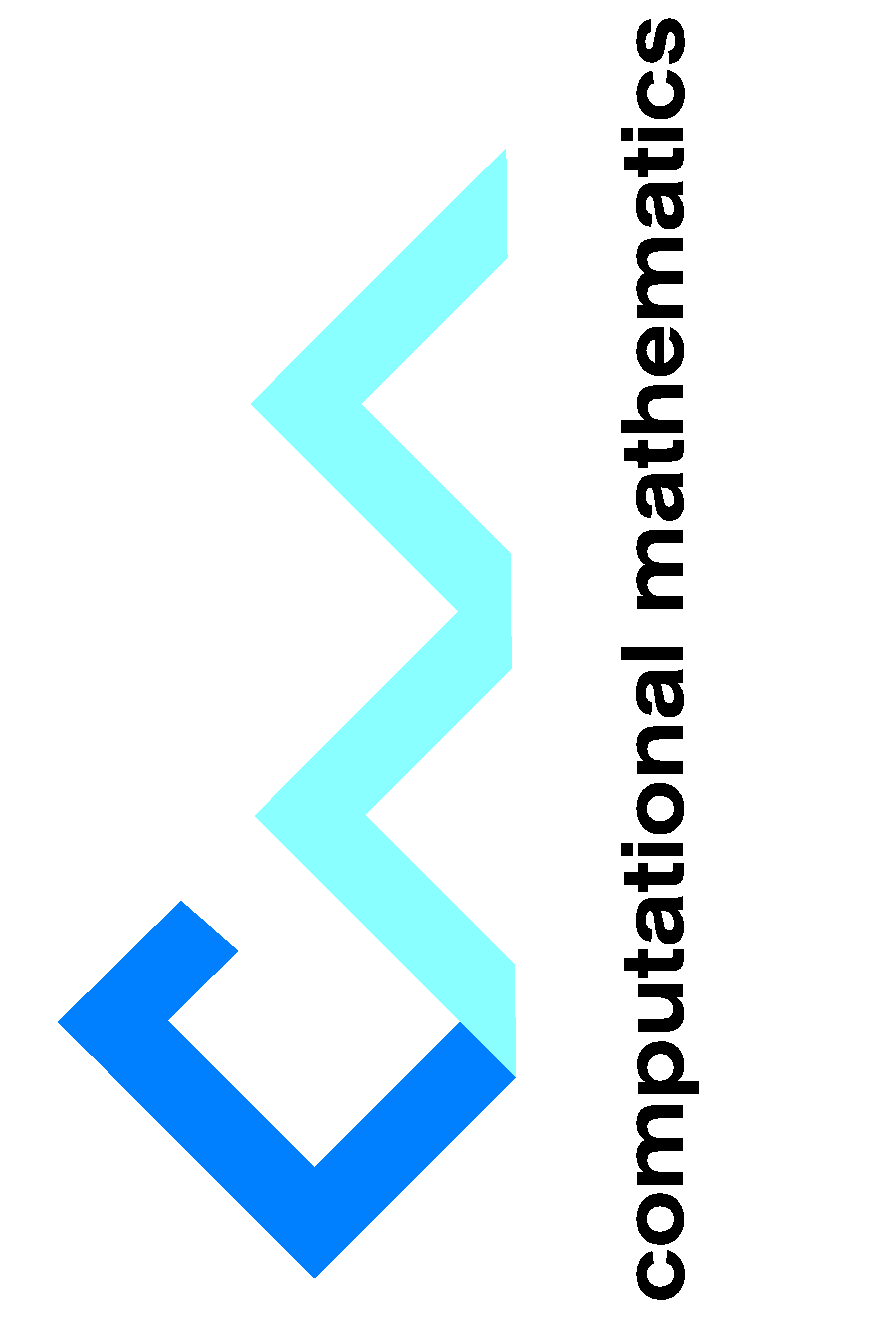
\includegraphics[width=.5\textwidth,angle=-90]{cm-logo2.eps} }   }   \\

\parbox{25ex}{
  Prof.~Dr.~S.~Sauter\\
  Institut f"ur Mathematik\\
  Universit"at Z"urich
  }
%
\rule[0cm]{0.cm}{.01cm}
\hfill  \parbox{0.6\textwidth}{
  {\sffamily\LARGE\bfseries Numerik I}
  {\sffamily\Large\bfseries \;\;--\;\; Homework \blnr }\\[1.5ex]
  Deadline: \sdate\ 13:00
  }
  
  
\vspace{10ex}

%%%%%%%%%%%%%%%%%%%%%%%%%%%%%%%%%%%%%%%%%%%%%%%%%%%%%%%%%%%%%%%%%%%%%%%%%%% 
% 
% Aufgaben 
% 
%%%%%%%%%%%%%%%%%%%%%%%%%%%%%%%%%%%%%%%%%%%%%%%%%%%%%%%%%%%%%%%%%%%%%%%%%%% 
\begin{aufg}[ Theoretical task]
\begin{enumerate}
\item (2 P.) Let $f \in C^0(\mathbb{R})$ be a continuous function. Suppose there exists some $X \in \mathbb{R}$ and $\varepsilon>0$, such that $[X-\varepsilon, X+\varepsilon]$ contains exactly one simple zero of $f$. Write an (efficient) algorithm to find real numbers $a$ and $b$ with $f(a)f(b)<0$.
\item (2 P.) Examine how the runtime of the algorithm depend on the unknowns $X$ and $\varepsilon$.
\end{enumerate}
\end{aufg}


\begin{aufg}[Computational task]
\begin{enumerate}
\item (1 P.) Implement the bisection method for finding zeros of a continuous function. 
\item (4 P.) Implement a method that finds the \(k\)-th zero (up to an accuracy of \(10^{-7}\)) of the Legendre polynomial \(P_n\) defined in Homework 7 Exercise 3. Test your program to find the \(8\)-th zero of \(P_{10}\).
\end{enumerate}
\end{aufg}

\begin{aufg}[Theoretical task, 3 P.]
Prove by induction the statement (7.6) (Separationseigenschaft) from the lecture notes.\\
Hint: Use the 3-term recursion formula and evaluate the polynomial \(\pi_{n+1}\) in the zeros of \(\pi_n\).
\end{aufg}

\begin{aufg}[Theoretical task]
We want to find the zeros of the function
\begin{align*}
f_a(x) = x^2-a
\end{align*}
using Newton's method.
\begin{enumerate}
\item (1 P.) How does the Newton iteration look like for this problem?
\item (3 P.) Prove that Newton's method converges to \(+\sqrt{a}\) for any positive starting value \(x_0\).
\end{enumerate}
\end{aufg}

\end{document}